\documentclass[tikz,border=8pt]{standalone}
\usepackage{amsmath}
\usepackage{pgfplots}
\pgfplotsset{compat=1.18}
\definecolor{ink}{HTML}{21352F}
\definecolor{teal}{HTML}{087F7B}
\definecolor{blue}{HTML}{4B77A8}
\definecolor{gold}{HTML}{C58B2A}
\definecolor{rose}{HTML}{B65A62}
\begin{document}
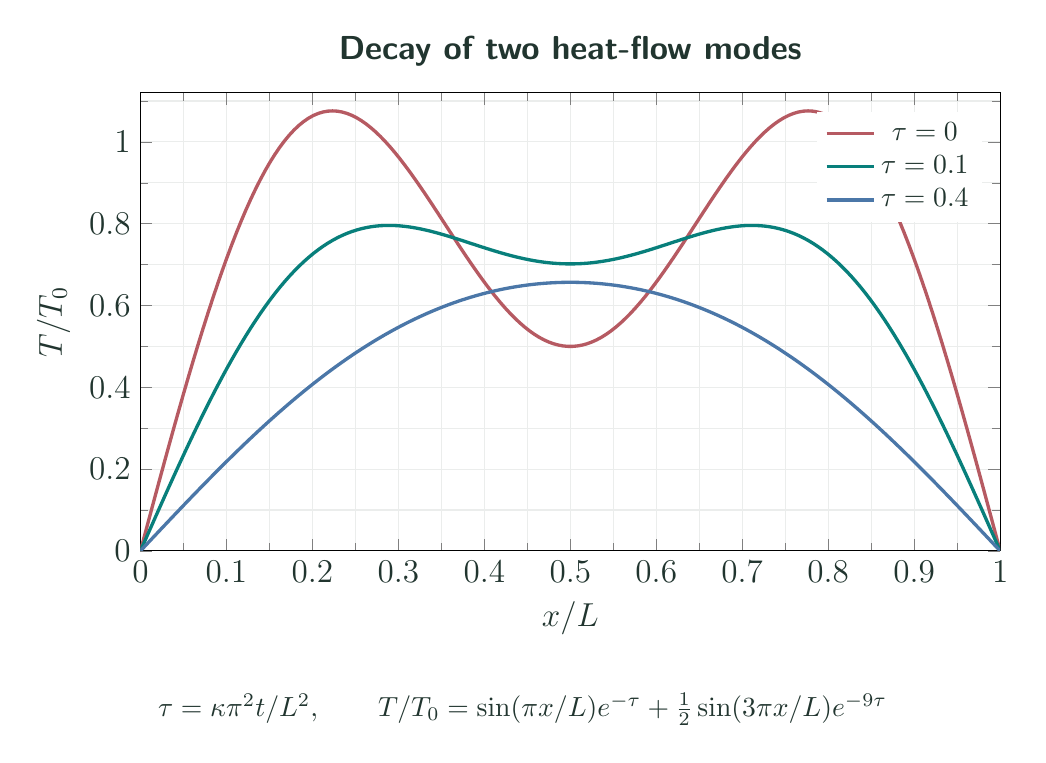
\begin{tikzpicture}[font=\large\sffamily,text=ink]
  \begin{axis}[
    width=12.5cm,height=7.4cm,
    xmin=0,xmax=1,ymin=0,ymax=1.12,
    xlabel={$x/L$},ylabel={$T/T_0$},
    samples=180,domain=0:1,
    grid=both,minor tick num=1,grid style={ink!9},
    title={\bfseries Decay of two heat-flow modes},
    legend style={draw=none,fill=white,at={(.98,.96)},anchor=north east,font=\normalsize}
  ]
    \addplot[rose,very thick]
      {sin(deg(pi*x))+.5*sin(deg(3*pi*x))};
    \addlegendentry{$\tau=0$}
    \addplot[teal,very thick]
      {sin(deg(pi*x))*exp(-.1)+.5*sin(deg(3*pi*x))*exp(-.9)};
    \addlegendentry{$\tau=0.1$}
    \addplot[blue,very thick]
      {sin(deg(pi*x))*exp(-.4)+.5*sin(deg(3*pi*x))*exp(-3.6)};
    \addlegendentry{$\tau=0.4$}
  \end{axis}
  \node[font=\normalsize,below=5mm] at (current bounding box.south)
    {$\tau=\kappa\pi^2t/L^2,\qquad
      T/T_0=\sin(\pi x/L)e^{-\tau}
      +\tfrac12\sin(3\pi x/L)e^{-9\tau}$};
\end{tikzpicture}
\end{document}
